\documentclass[11pt, a4paper]{scrartcl}
\usepackage[ngerman]{babel}
%\usepackage[T1]{fontenc}
\usepackage[utf8]{inputenc}
\usepackage{lmodern}
\usepackage{amsmath}
\usepackage{amssymb}
\usepackage{amsthm}
\usepackage{graphicx}
\usepackage{listings}
\usepackage{booktabs}
\usepackage{float}
\usepackage{pdfpages}
\usepackage{cite}
\usepackage{url}
\bibliographystyle{unsrtnat}
\usepackage[numbers]{natbib}
\usepackage[T1]{fontenc}
%
\begin{document}
\lstset{basicstyle=\small,
		 inputencoding=latin1,
		stringstyle=\ttfamily,
		identifierstyle=,
		showstringspaces=false,
		language=c,
		frame=trBL}
%
\subsection*{TI III WS 2013, Fr. 12-14}
\section*{Lösung Übungsblatt 5}
\textbf{Christoph van Heteren-Frese (Matr.-Nr.: 4465677), Julien  Stengel } \\%(Matr.-Nr.: 4567553)}\\
Tutor: Ruhland, eingereicht am \today\\
\hrule
%
\section*{Aufgabe 2}
\subsection*{a)}
\begin{figure}[H]
\center
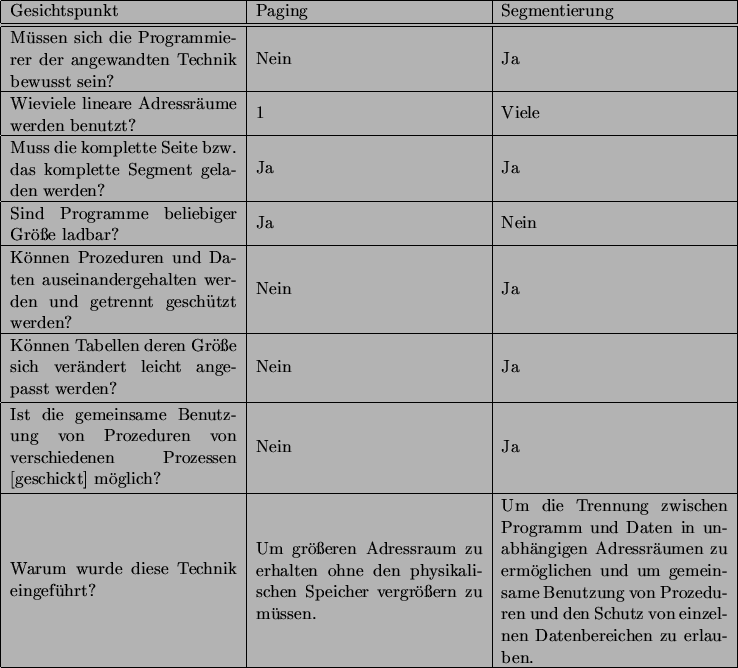
\includegraphics[scale=0.55]{img18}
\caption{Vergleich von Paging und Segmentierung aus \citep{tanenbaum_moderne_1994}}
\end{figure}
\subsection*{b)}
\subsection*{c)}
\section*{Aufgabe 4}
\subsection*{a)} 
Der Operator \texttt{!=} (\textit{not equal to}, Prioritätsstufe 9) bindet stärker als \texttt{=} (\textit{direct assignment}, Prioritätsstufe 16). Daher müssen wie folgt Klammern gesetzt werden:
\begin{lstlisting}
while ( (c = getchar ()) != EOF )
	putchar ( c );
\end{lstlisting}
%\lstinputlisting{../u4_4.c}
\subsection*{b)}
Es wird ein Zahlenpaar ausgegeben. Die zweite Zahl ist dabei die Quadratzahl des direkten Vorgängers der erste Zahl. Diese Ausgabe entspricht warscheinlich nicht der Intention des Programierers. \\

\noindent
\textbf{Begründung:} Erscheint der Opperator \texttt{++} vor dem Operand, wird dessen Wert zunächst inkrementiert und erst dann in  dem Ausdruck benutzt. Steht \texttt{++} hinter dem Operand, wird sein aktueller Wert erst im Ausdruck benutzt und anschließend inkrementiert.
%Die funktion \texttt{pow()} liefert einen Wert vom Typ \textit{double} zurück.
\subsection*{c)}
\begin{enumerate}
\item Der Wert von \texttt{len} wird inkrementiert. \\
\texttt{->} bindet stärker (Prioritätsstufe 2) als \texttt{++} (Prioritätsstufe 3). Daher wird zuerst \texttt{p->len} ausgewertet (\texttt{p->len} ist äquivalent mit \texttt{(*p).len}) und somit auf die Variable \texttt{len} der Struktur \texttt{p} zugegriffen. Diese wird anschließend inkrementiert.
\item Hier wird erst der Zeiger \texttt{p} inkrementiert und dann auf das Element len der Struktur zugegriffen, auf den der nächste Zeiger zeigt.
\item
\item Der Wert von \texttt{str} wird inkrementiert.
\item

\end{enumerate}
\subsection*{d)}
\subsection*{e)}
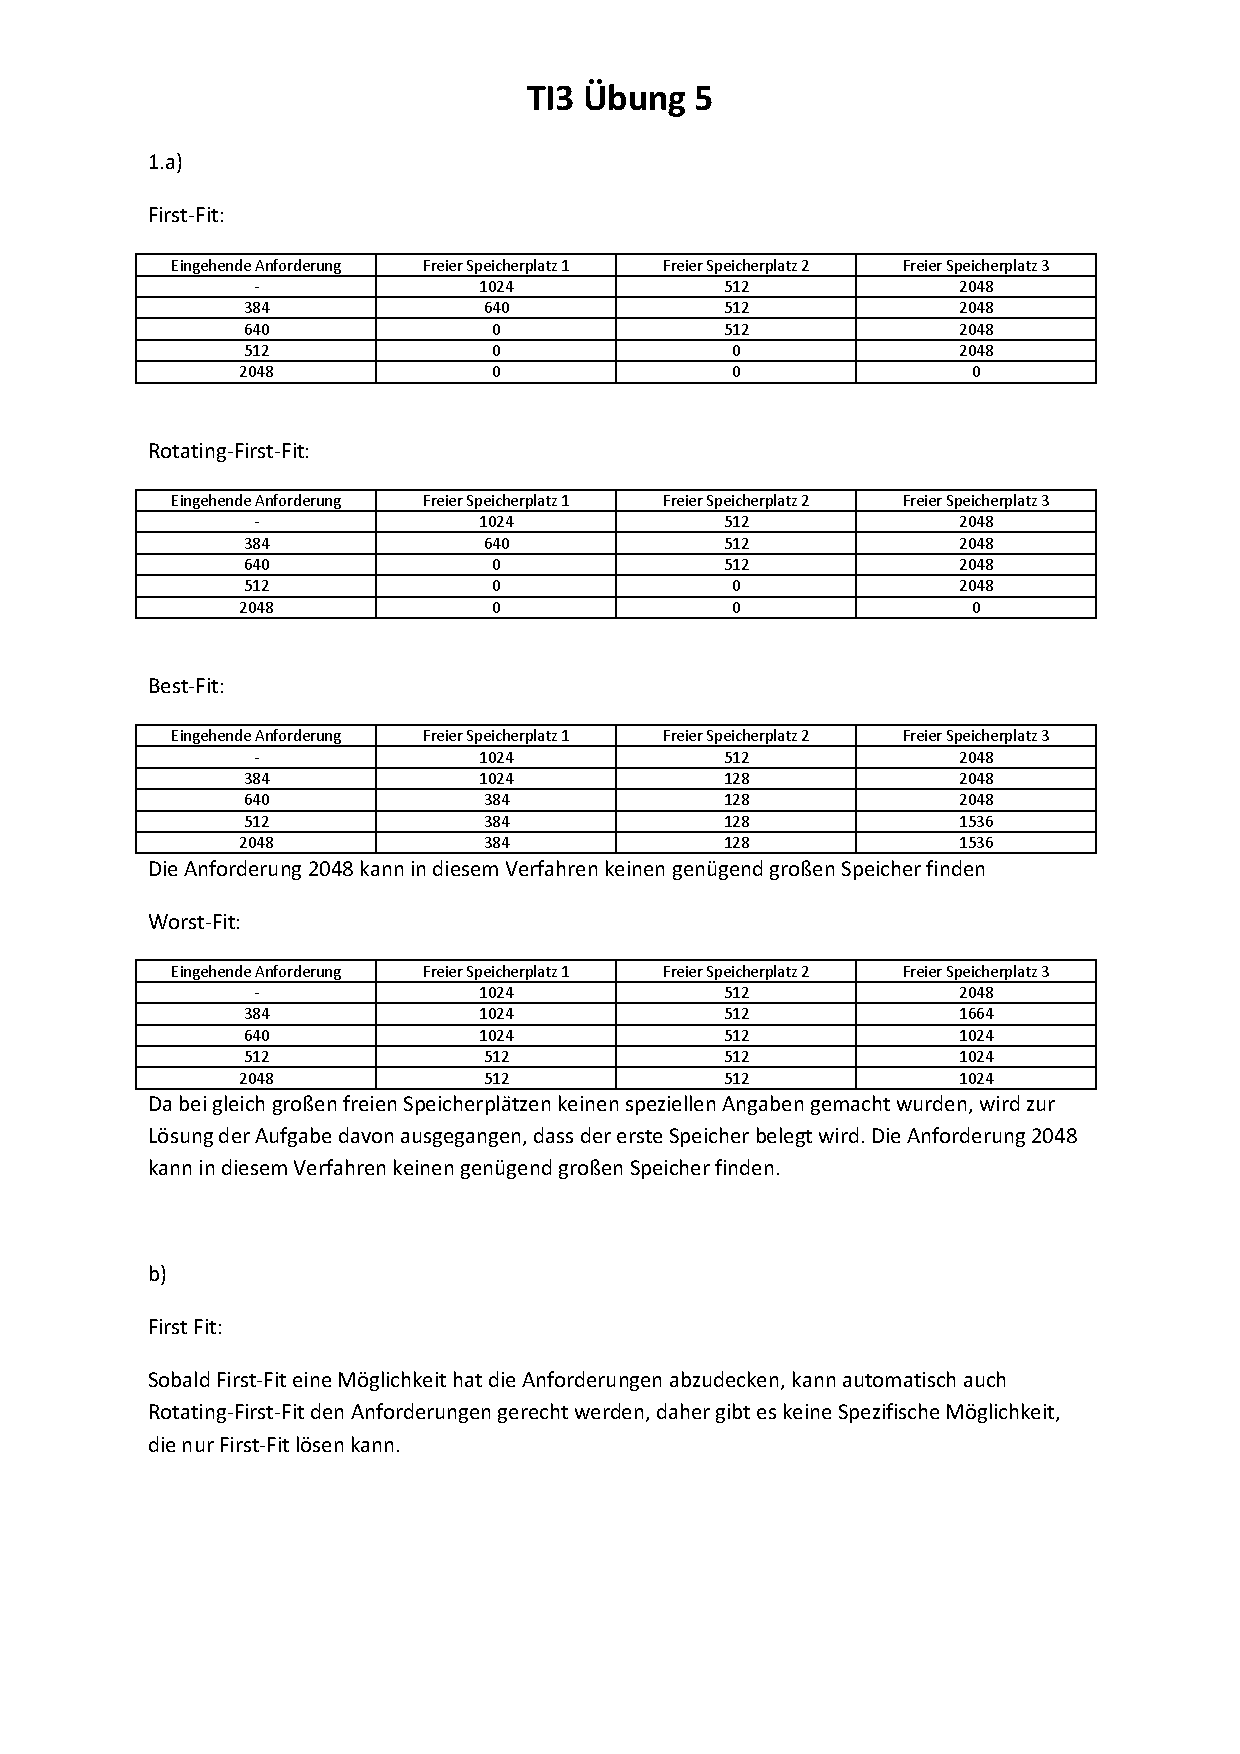
\includepdf[pages={1,2}]{../Uebung5.pdf}
\bibliography{ti3}
\end{document}
